\documentclass{anstrans}
%%%%%%%%%%%%%%%%%%%%%%%%%%%%%%%%%%%
\title{Energy alternatives to reduce the University of Illinois at Urbana-Champaign campus CO$_2$ emissions}
\author{Roberto E. Fairhurst Agosta, Tomasz Kozlowski}

\institute{
University of Illinois at Urbana-Champaign, Dept. of Nuclear, Plasma, and Radiological Engineering\\
ref3@illinois.edu
}

%%%% packages and definitions (optional)
\usepackage{graphicx} % allows inclusion of graphics
\usepackage{booktabs} % nice rules (thick lines) for tables
\usepackage{microtype} % improves typography for PDF
\usepackage{xspace}
\usepackage{tabularx}
\usepackage{caption}
\usepackage{floatrow}
\usepackage{subcaption}
\usepackage{enumitem}
\usepackage{placeins}
\usepackage{amsmath}
\usepackage[acronym,toc]{glossaries}
\newacronym{ANL}{ANL}{Argonne National Laboratory}
\newacronym{API}{API}{Application Programming Interface}
\newacronym{ATR}{ATR}{Advanced Test Reactor}
\newacronym{B4C}{B4C}{boron carbide}
\newacronym{BC}{BC}{boundary condition}
\newacronym{BOC}{BOC}{beginning of the equilibrium cycle}
\newacronym{BSD}{BSD}{Berkeley Software Distribution}
\newacronym{BWR}{BWR}{Boiling Water Reactor}
\newacronym{CAISO}{CAISO}{California ISO}
\newacronym{CAPP}{CAPP}{Core Analyzer for Pebble and Prism type VHTRs}
\newacronym{CEA}{CEA}{Commissariat a l'Energie Atomique}
\newacronym{CFD}{CFD}{computational fluid dynamics}
\newacronym{CO2}{CO$_2$}{carbon dioxide}
\newacronym{CNN}{CNN}{convolutional neural network}
\newacronym{CR}{CR}{control rod}
\newacronym{CRP}{CRP}{Coordinated Research Project}
\newacronym{CZP}{CZP}{Cold Zero Power}
\newacronym{DCC}{DCC}{depressurized conduction cool-down}
\newacronym{DOE}{DOE}{Department of Energy}
\newacronym[\glslongpluralkey={degrees of freedom}]{DoF}{DoF}{degree of freedom}
\newacronym{DT}{DT}{decision tree}
\newacronym{DTR}{DTR}{decision tree regression}
\newacronym{EOC}{EOEC}{end of the equilibrium cycle}
\newacronym{FCEV}{FCEV}{Fuel Cell Electric Vehicle}
\newacronym{FDM}{FDM}{Finite Difference Method}
\newacronym{FEM}{FEM}{Finite Element Method}
\newacronym{FNN}{FNN}{feedforward neural network}
\newacronym{FVM}{FVM}{Finite Volume Method}
\newacronym[\glslongpluralkey={greenhouse gases}]{GHG}{GHG}{greenhouse gas}
\newacronym[\glslongpluralkey={Gaussian processes}]{GP}{GP}{Gaussian process}
\newacronym{GRS}{GRS}{Gesellschaft für Anlagen und Reaktorsicherheit}
\newacronym{GT-MHR}{GT-MHR}{Gas Turbine-Modular Helium Reactor}
\newacronym{H2}{H$_2$}{hydrogen}
\newacronym{He}{He}{helium}
\newacronym{HFP}{HFP}{Hot Full Power}
\newacronym{HPCC}{HPCC}{high-pressure conduction cool-down}
\newacronym{HTE}{HTE}{High-Temperature Electrolysis}
\newacronym{HTGR}{HTGR}{High-Temperature Gas-Cooled Reactor}
\newacronym{HTR}{HTR}{High Temperature Reactor}
\newacronym{HTTR}{HTTR}{High-Temperature engineering Test Reactor}
\newacronym{HZDR}{HZDR}{Helmholtz-Zentrum Dresden-Rossendorf}
\newacronym{IAEA}{IAEA}{International Atomic Energy Agency}
\newacronym{icap}{iCAP}{Illinois Climate Action Plan}
\newacronym{INL}{INL}{Idaho National Laboratory}
\newacronym{IPyC}{IPyC}{inner pyrolytic carbon}
\newacronym{JFNK}{JFNK}{Jacobian-Free Newton-Krylov}
\newacronym{KAERI}{KAERI}{Korea Atomic Energy Research Institute}
\newacronym{Keff}{k$_{eff}$}{multiplication factor}
\newacronym{KNN}{KNN}{K-Nearest Neighbor}
\newacronym{LBP}{LBP}{Lumped Burnable Poison}
\newacronym{LGPL}{LGPL}{Lesser GNU Public License}
\newacronym{LOCA}{LOCA}{loss-of-coolant accident}
\newacronym{LOFW}{LOFW}{loss of feedwater}
\newacronym{LogR}{LogR}{Logistic Regression}
\newacronym{LPCC}{LPCC}{low-pressure conduction cool-down}
\newacronym{LSTM}{LSTM}{long short-term memory}
\newacronym{LTE}{LTE}{Low-Temperature Electrolysis}
\newacronym{LWR}{LWR}{Light Water Reactor}
\newacronym{MC}{MC}{Monte Carlo}
\newacronym{MHTGR}{MHTGR}{Modular High-Temperature Gas-Cooled Reactor}
\newacronym{ML}{ML}{machine learning}
\newacronym{MMR}{MMR}{Micro Modular Reactor}
\newacronym{MOC}{MOC}{middle of the equilibrium cycle}
\newacronym{MOX}{MOX}{Mixed-Oxide}
\newacronym{MOOSE}{MOOSE}{Multi-physics Object-Oriented Simulation Environment}
\newacronym{MPI}{MPI}{Message Passing Interface}
\newacronym{MSE}{MSE}{mean squared error}
\newacronym{MSR}{MSR}{Molten Salt Reactor}
\newacronym{MTD}{MTD}{Champaign-Urbana Mass Transit District}
\newacronym{NEA}{NEA}{Nuclear Energy Agency}
\newacronym{NEM}{NEM}{Nodal Expansion Method}
\newacronym{NGNP}{NGNP}{Next Generation Nuclear Power}
\newacronym{NRC}{NRC}{Nuclear Regulatory Commission}
\newacronym{NSC}{NSC}{Nuclear Science Committee}
\newacronym{OECD}{OECD}{Organisation for Economic Co-operation and Development}
\newacronym{OPyC}{OPyC}{outer pyrolytic carbon}
\newacronym{ORNL}{ORNL}{Oak Ridge National Laboratory}
\newacronym{OS}{OS}{Operator-Splitting}
\newacronym{PBMR}{PBMR}{Pebble Bed Modular Reactor}
\newacronym{PDE}{PDE}{Partial Differential Equation}
\newacronym{PMR}{PMR}{Prismatic Modular Reactor}
\newacronym{PV}{PV}{photovoltaics}
\newacronym{RFR}{RFR}{random forest regression}
\newacronym{RF}{RF}{random forest}
\newacronym{RPV}{RPV}{Reactor Pressure Vessel}
\newacronym{RSC}{RSC}{Reserve Shutdown Control}
\newacronym{RSD}{RSD}{Relative Standard Deviation}
\newacronym{SD}{SD}{Standard Deviation}
\newacronym{SI}{SI}{Sulfur-Iodine}
\newacronym{SiC}{SiC}{silicon carbide}
\newacronym{SMR}{SMR}{Small Modular Reactor}
\newacronym{SNU}{SNU}{Seoul National University}
\newacronym{SOEC}{SOEC}{Solid Oxide Electrolysis Cells}
\newacronym{SP3}{SP$_3$}{Simplified P$_3$}
\newacronym{SVM}{SVM}{support vector machine}
\newacronym{SVR}{SVR}{support vector regression}
\newacronym{TIP}{TIP}{transverse integration procedure}
\newacronym{TRISO}{TRISO}{Tristructural Isotropic}
\newacronym{UIUC}{UIUC}{University of Illinois at Urbana-Champaign}
\newacronym{UNIST}{UNIST}{Ulsan National Institute of Science and Technology}
\newacronym{UK}{UK}{United Kingdom}
\newacronym{UMICH}{UMICH}{University of Michigan}
\newacronym{US}{US}{United States}
\newacronym{USNC}{USNC}{Ultra Safe Nuclear Corporation}
\newacronym{VHTR}{VHTR}{Very High-Temperature Gas-Cooled Reactor}
\newacronym{WRM}{WRM}{weighted residual method}
%\newacronym{<++>}{<++>}{<++>}
%\newacronym{<++>}{<++>}{<++>}
% \makeglossaries

\usepackage[printwatermark]{xwatermark}
\usepackage{xcolor}
\usepackage{graphicx}
\usepackage{lipsum}


\renewcommand{\vec}[1]{\bm{#1}} %vector is bold italic
\newcommand{\vd}{\bm{\cdot}} % slightly bold vector dot
\newcommand{\grad}{\vec{\nabla}} % gradient
\newcommand{\ud}{\mathop{}\!\mathrm{d}} % upright derivative symbol

\newcolumntype{c}{>{\hsize=.56\hsize}X}
\newcolumntype{b}{>{\hsize=.7\hsize}X}
\newcolumntype{s}{>{\hsize=.74\hsize}X}
\newcolumntype{f}{>{\hsize=.1\hsize}X}
\newcolumntype{a}{>{\hsize=.45\hsize}X}
%\usepackage[pagestyles]{titlesec}
%\titleformat*{\subsection}{\normalfont}
%\titleformat{\section}{\bfseries}{Item \thesection.\ }{0pt}{}

%\newwatermark[allpages,color=gray!50,angle=45,scale=3,xpos=0,ypos=0]{DRAFT}

\begin{document}
%%%%%%%%%%%%%%%%%%%%%%%%%%%%%%%%%%%%%%%%%%%%%%%%%%%%%%%%%%%%%%%%%%%%%%%%%%%%%%%%


\section{Introduction}

% Motivation: Why is decarbonization necessary
Energy is one of the major contributors to economic growth.
In the future, economies and populations will continue to expand, and their energy demand will accompany such a change.
Meeting these future needs requires the addition of energy sources into the grid.
In 2019, electricity generation was one of the economic sectors that released the most \glspl{GHG} in the US \cite{us_epa_sources_2015}.
Decarbonizing electricity generation will allow us to meet the increases in demand and address the environmental concerns simultaneously.
% Incorporating carbon-free energy sources will allow us to meet the increases in demand and address the environmental concerns simultaneously.

\begin{figure}[htbp!] %or H 
    \centering
    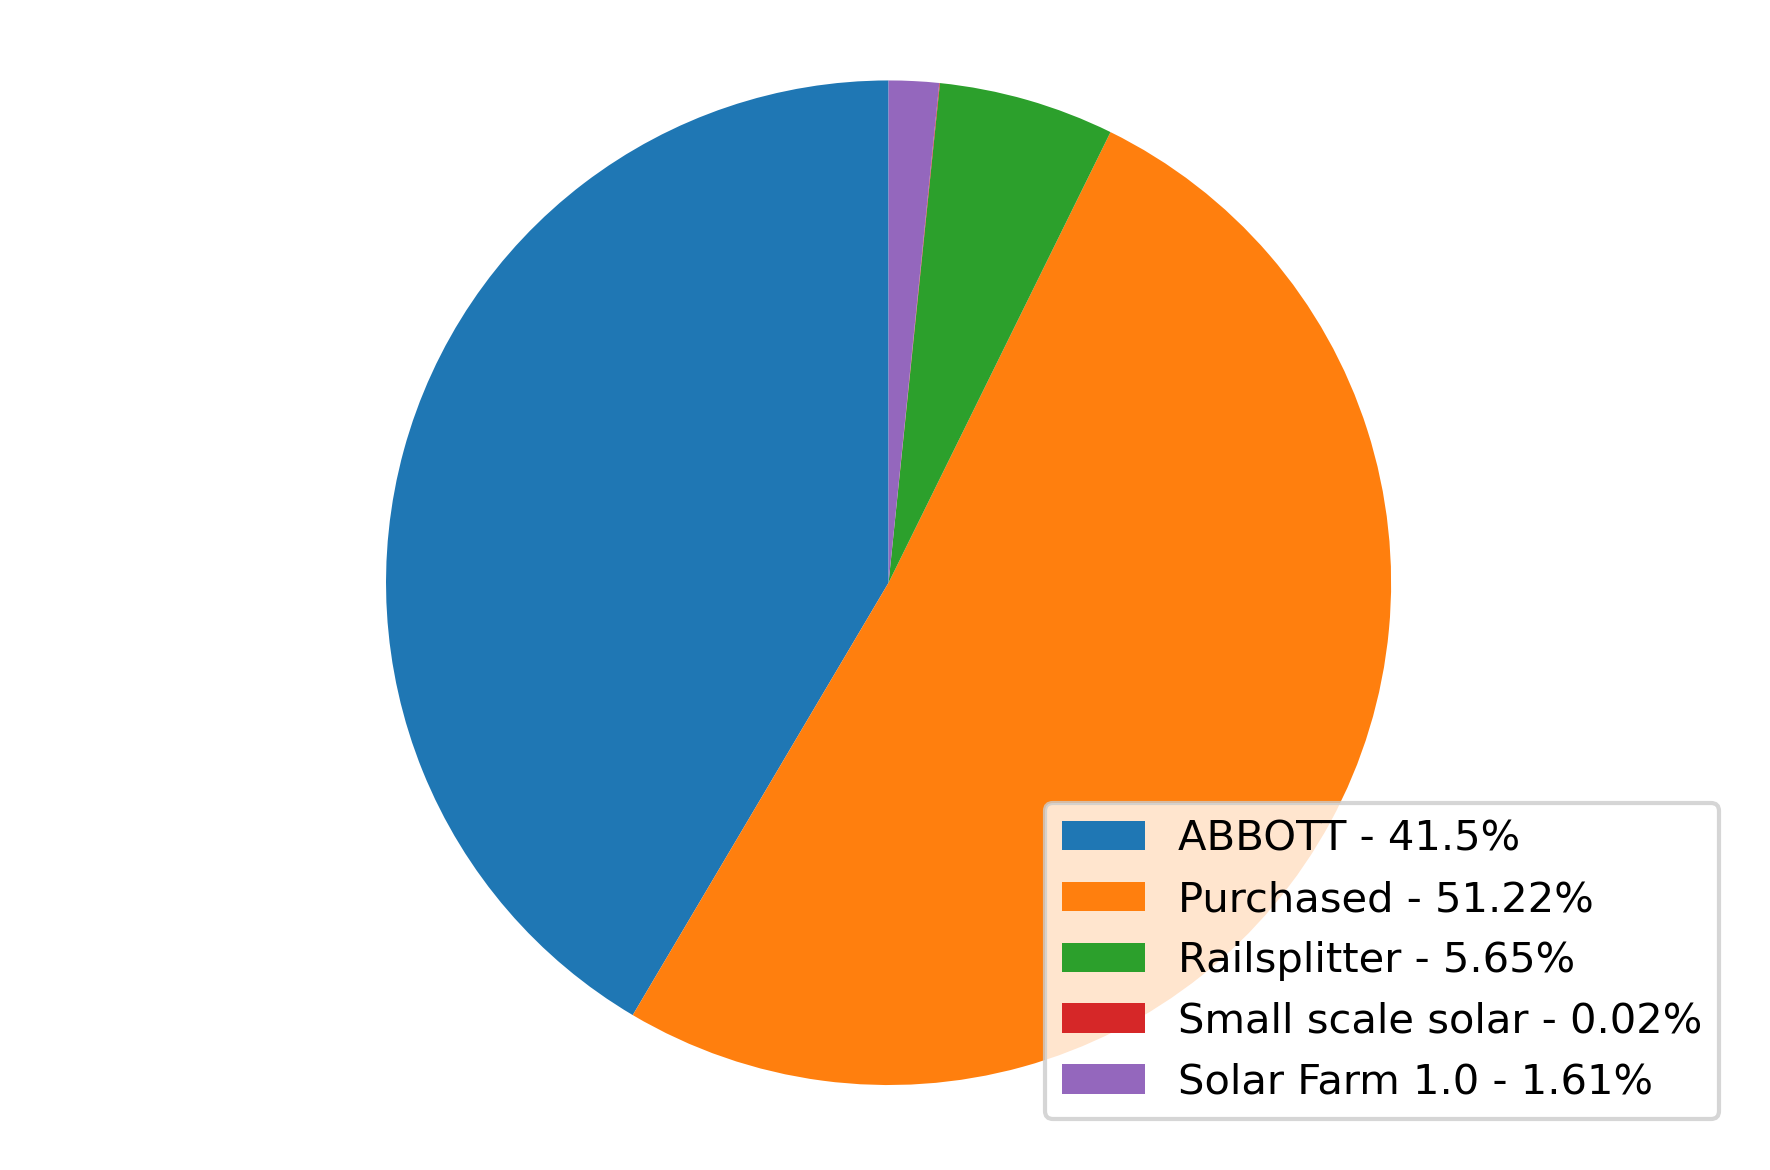
\includegraphics[width=0.90\linewidth]{figures/elec-distrib}
    \hfill
    \caption{Distribution of electricity generation of UIUC campus in fiscal year 2019 \cite{isee_illinois_2020}.}
    \label{fig:elec-distrib}
\end{figure}

% UIUC
% This work focuses on the decarbonization of UIUC campus grid, aligning its objectives with the Illinois Climate Action Plan (iCAP) \cite{institute_for_sustainability_energy_and_environment_illinois_2015, institute_for_sustainability_energy_and_environment_illinois_2020}.
% In 2008, UIUC signed the American College and University Presidents’ Climate Commitment, formally committing to becoming carbon neutral as soon as possible, no later than 2050.
% The university developed the iCAP in 2010 as a comprehensive roadmap toward a sustainable campus environment.

This work studies several energy alternatives for decarbonizing the \gls{UIUC} campus grid.
The alternatives presented here can be extrapolated to any other grid.
We focus on the \gls{UIUC} campus grid because it is a well-characterized grid integrating a diverse mix of energy sources, as shown in Figure \ref{fig:elec-distrib}.
% Campus Grid
%% Abbott
The Abbott Power Plant is a co-generation facility that supplies the campus with electricity and steam.
The plant has multiple gas turbines and boilers that run on natural gas, fuel oil, or coal.
The production of high-pressure steam spins a turbine to drive a generator and produce electricity.
The low-pressure exhaust steam fulfills the space heating, water heating, and space cooling requirements from campus.
Abbott’s maximum capacity is 85 MW for electricity and 800 klbs/h for steam \cite{uiucfs_abbott_nodate}.
%% Purchased
To provide cost-effective utilities, the university purchases electricity with the assistance of a market advisor \cite{uiucfs_energy_2015}.
%% Wind
The Rail Splitter Wind Farm has 67 wind turbines of 1.5 MW each, providing the farm a maximum power output of 100.5 MW.
Through a power purchase agreement, the university buys 8.6\% of the wind farm's total generation \cite{rail_splitter_illinois_2016, uiucfs_energy_2015}.
%% Solar
The Solar Farm 1.0 comprises 18,867 modules, which cover a land area of 20.8 acres and produce a power output of 4.68 MW \cite{uiucfs_solar_2017}.
The small-scale solar generation comprises all the solar generation distributed around campus, considered negligible in this work.

% Objectives
The main objective of this work is to analyze multiple electricity generation alternatives for decreasing CO$_2$ emissions on the UIUC campus.
For this reason, this paper evaluates two scenarios increasing the wind and solar generation capacity.
The second scenario also considers the addition of a nuclear reactor into the mix.
Due to the non-dispatchable nature of wind and solar generation, both scenarios incorporate electricity storage mechanisms.


\section{Electricity Storage Mechanisms}

This work considers two storage mechanisms, Li-ion batteries, and hydrogen produced via electrolysis of water.
This section briefly describes each of them and their integration into the grid.

% Li-ion
The first prototype of a Li-ion battery was developed in 1985, becoming recently popular in the last two decades.
Li-ion batteries are rechargeable and are commonly used in laptops, cellphones, electric vehicles, Uninterruptible Power Supplies (UPS), and for communication and medical applications.
A high energy density and low self-discharge characterize this type of battery.
Additionally, its charge-discharge efficiency of 80-90\% makes it a good candidate for electricity storage \cite{sun_car_2010}.
This work considers the charge-discharge efficiency of Li-ion batteries to be 85\%.

% Hydrogen
The electrolysis of water is a well-known process whose commercial use began in 1890.
This process produces approximately 4\% of the worldwide hydrogen.
% The process is ecologically clean because it does not emit GHGs.
% However, in comparison with other methods, electrolysis is a highly energy-demanding technology.
Three electrolysis technologies exist.
Alkaline-based is the most common, the most developed, the lowest in capital cost, and the least efficient.
Proton exchange membrane (PEM) electrolyzers are more efficient but more expensive than Alkaline electrolyzers.
Solid Oxide Electrolysis Cells (SOEC) electrolyzers are the most electrically efficient but the least developed.
% SOEC technology has challenges with corrosion, seals, thermal cycling, and chrome migration.
The first two technologies work with liquid water, and the latter requires high-temperature steam.
This work refers to the first two technologies as \gls{LTE} and the latter as \gls{HTE} \cite{fairhurst-agosta_multi-physics_2020}.

% Still Hydrogen
Water electrolysis converts electric and thermal energy into chemical energy stored in hydrogen.
The process enthalpy change $\Delta H$ determines the required energy for the electrolysis reaction to take place
\begin{align}
  \Delta H = \Delta G + T \Delta S
\end{align}
where $\Delta G$ is the specific electrical energy and $T \Delta S$, the specific thermal energy.
In LTE, electricity generates the necessary thermal energy.
Hence, $\Delta G$ determines the entire process’s energy requirement.
$\Delta G$ is equal to 60 kWh/kg-H$_2$ considering a 67\% electrolyzer electrical efficiency.
In HTE, a high-temperature heat source provides the necessary thermal energy.
$\Delta G$ decreases with increasing temperatures, as shown in Figure \ref{fig:hte-energy}.
% Decreasing the electricity requirement results in higher overall production efficiencies since heat-engine-based electrical work has a thermal efficiency of 50\% or less.
Decreasing the electricity requirement results in higher overall production efficiencies.
This work considers the process to be at 3.5 MPa.
Although $\Delta G$ increases with pressure, a high pressure saves energy, as compressing liquid water is cheaper than compressing the hydrogen.
In his work, $\Delta G$ and $T \Delta S$ are 31.6 and 9.7 kWh/kg-H$_2$, respectively, for a reactor outlet temperature of 850 $^\circ$C.
% In his work, $\Delta G$ and $T \Delta S$ are 31.6 and 9.7 kWh/kg-H$_2$ for an electrolysis temperature of 824.5 $^\circ$C, respectively.
% This work considers a reactor outlet temperature of 850 and an efficiency of 97%, 0.97*850 = 824.5

\begin{figure}[htbp!] %or H 
    \centering
    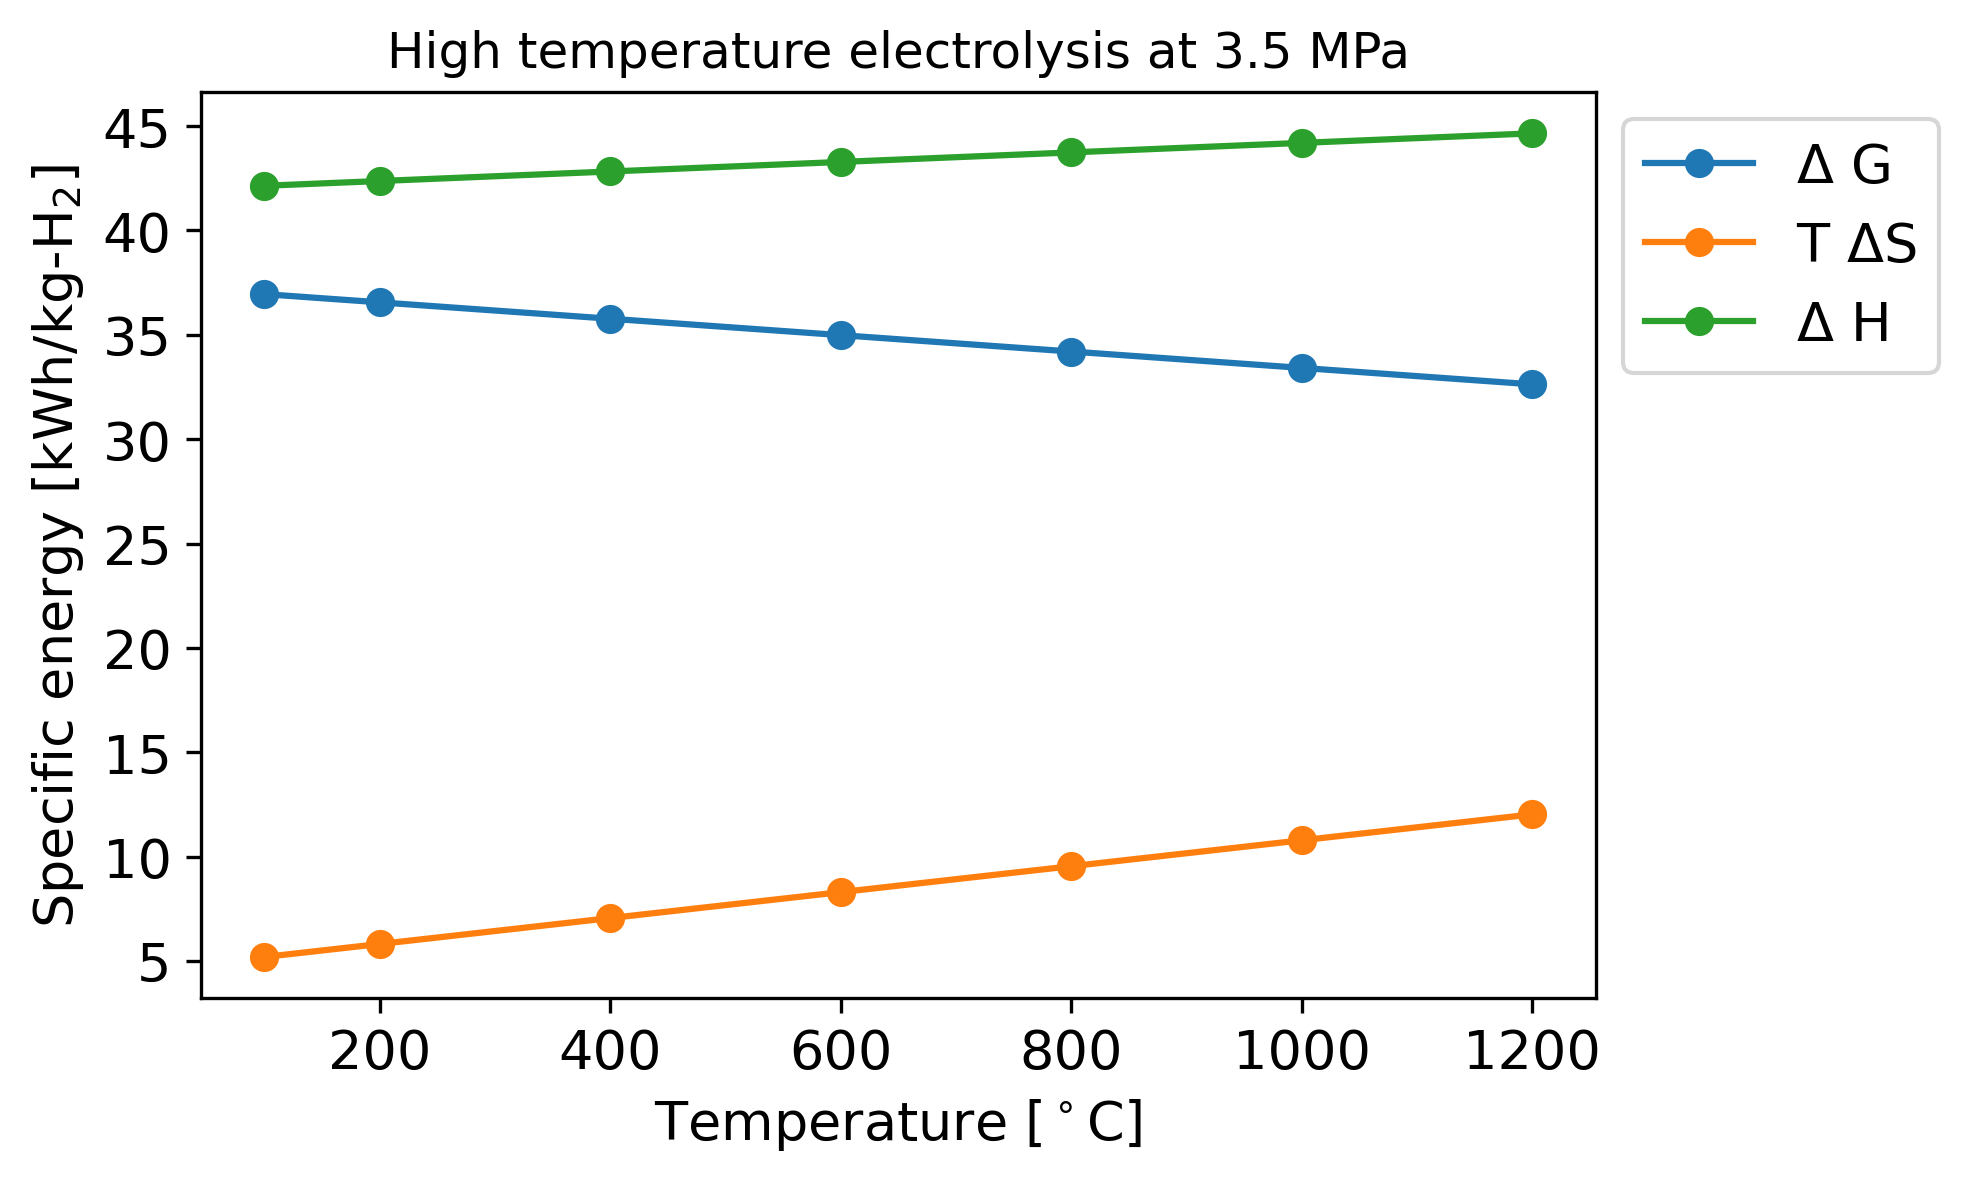
\includegraphics[width=0.90\linewidth]{figures/hte-energy-P}
    \hfill
    \caption{Energy required by high-temperature electrolysis at 3.5 MPa. Image reproduced from \cite{fairhurst-agosta_multi-physics_2020}.}
    \label{fig:hte-energy}
\end{figure}

After converting the excess energy into hydrogen, it is stored until the grid requires it.
The conversion of hydrogen produces 40 kWh/kg-H$_2$ \cite{ursua_hydrogen_2012}.
However, conventional fuel cells can use up to 60\% of that energy \cite{doe_energy_fuel_2015}.


\section{Methodology}

As mentioned earlier, the focus of this paper is to decrease the CO$_2$ emissions on the UIUC campus.
This paper studies two energy alternatives, Scenario 1 and 2, and compares them to the default case, Scenario 0.

\textbf{Scenario 0} considers the business as usual case.
We calculate the CO$_2$ emissions using the electricity production hourly data.
These data are available per request from UIUC Facilities and Services.
To narrow down the scope, we focus on months of the two most demanding seasons of the year, January for the winter and June for the summer.
% Abbott and the purchased electricity are estimated to emit 0.26 tCO$_2$/MW(th)h and 0.825 tCO$_2$/MWh, respectively \cite{isee_illinois_2015, isee_illinois_2020}.
% I haven't mentioned that we consider abbot to have a thermal efficiency of 60 \%
% Abbott: 0.26 * 0.907185 / 0.6 /// Purchases: 0.825 * 0.907185
Abbott and the purchased electricity are estimated to emit 0.39 MT CO$_2$/MWh and 0.75 MT CO$_2$/MWh, respectively \cite{isee_illinois_2015, isee_illinois_2020}.

\textbf{Scenario 1} studies the increase of the wind and solar generation capacity up to ten times fold.
The increase in the wind and solar generation capacity requires the addition of electricity storage mechanisms into the mix.
The development of a dispatch model is necessary to calculate the energy being stored, Abbott hourly production, and the purchased electricity.
This model gives priority to the different sources in the following order: wind and solar, storage mechanism, Abbott, and purchases, as shown in Figure \ref{fig:dispatch-model}.
The \gls{ND} is calculated by subtracting the wind and solar generation from the total demand.
Abbott’s electricity generation is preferred over purchases because of their lower CO$_2$ emissions.

\begin{figure}[htbp!] %or H 
    \centering
    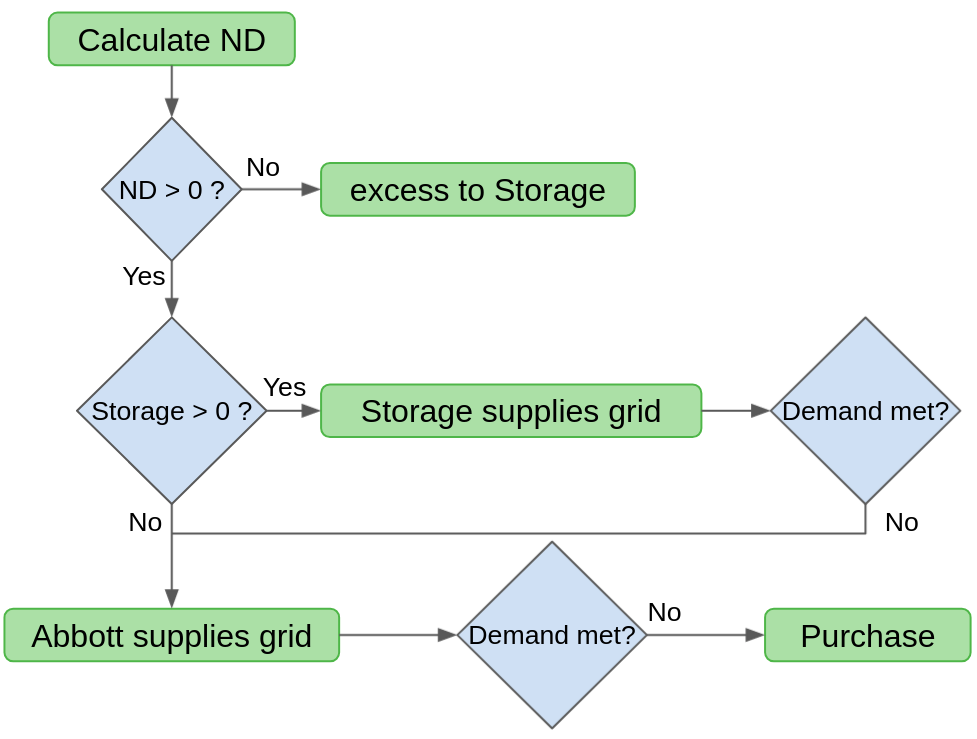
\includegraphics[width=0.90\linewidth]{figures/dispatch-model}
    \hfill
    \caption{Scenario 1 and 2 dispatch model that calculates the hourly generation of the different sources. \textit{ND} is the net demand.}
    \label{fig:dispatch-model}
\end{figure}

\textbf{Scenario 2} is similar to Scenario 1 but considers the addition of a nuclear reactor into the mix.
This model gives priority to the different sources in the following order: wind and solar, nuclear reactor, storage mechanism, Abbott, and purchases.
The \gls{ND} is calculated by subtracting the wind, solar, and nuclear generation from the total demand.
Given that UIUC campus demand is typically smaller than 80 MW, the following analyses consider reactors of small capacities, such as microreactors.
This type of reactor shows several advantages such as requiring limited on-site preparation as their components are factory-fabricated and shipped out to the generation site.
Moreover, these reactors use passive safety systems, minimizing electrical parts \cite{us-doe_ultimate_2019}.
% They allow for black starts, being capable of starting up from an utterly de-energized state without receiving power from the grid.
% They can also operate in islanding mode, being able to operate connected to the grid or independently.

This scenario considers 2 reactor power levels, 10 and 20 MW$_{th}$, and 2 reactor outlet temperatures, 300 and 850 $^\circ$C.
Conventional \glspl{LWR} -- with outlet temperatures of 300 $^\circ$C -- have efficiencies around 33\% while Gen-IV reactors, for example, \glspl{VHTR} -- with outlet temperatures of 850 $^\circ$C -- can achieve higher efficiencies around 48\% \cite{fairhurst-agosta_multi-physics_2020}.

Depending on the preferred electrolysis method, the microreactor can supply the hydrogen plant with both electricity and thermal power, as shown in Figure \ref{fig:reactor-hydrogen}, where $\eta$ is the thermal-to-electric conversion efficiency, and $\beta$ and $\gamma$ determine the distribution of the reactor thermal power P$_{th}$ into P$_E$, P$_{EH2}$, and P$_{TH2}$.
P$_E$ is calculated by the dispatch model.
The following formulas allow to calculate all the rest of the model variables

\begin{align}
  \beta = \frac{P_{E}}{\eta P_{th}}&, \; \gamma = \frac{\Delta G / \eta}{\Delta G / \eta + T \Delta S} \\
  \dot{m_{H2}} &= \frac{\gamma (1-\beta) \eta P_{th}}{\Delta G} \\
  P_{EH2} = \dot{m_{H2}} \Delta G&, \;  P_{TH2} = \dot{m_{H2}} T \Delta S
\end{align}

where $\dot{m_{H2}}$ is the hydrogen production rate.
This work considers an $\eta$ of 0.32 for a reactor outlet of 300 $^\circ$C and 0.49 for a reactor outlet of 850 $^\circ$C.

\begin{figure}[htbp!] %or H 
    \centering
    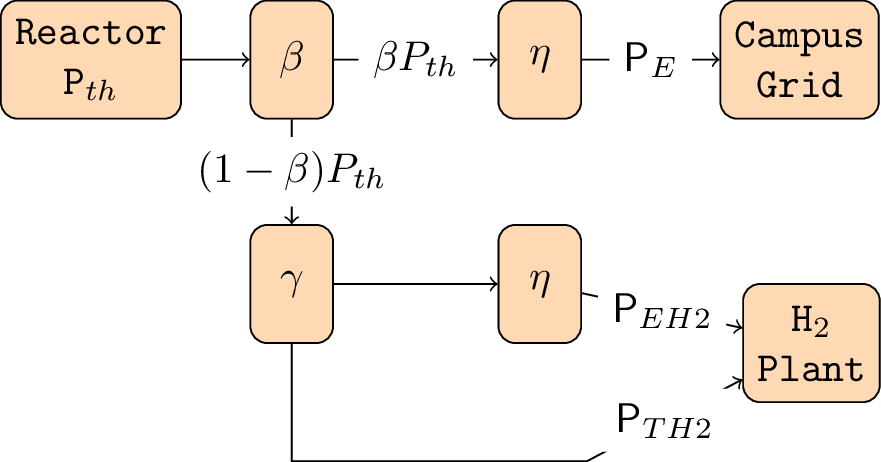
\includegraphics[width=0.90\linewidth]{figures/reactor-hydrogen}
    \hfill
    \caption{Diagram of a nuclear reactor supplying the grid and a hydrogen plant.}
    \label{fig:reactor-hydrogen}
\end{figure}

Only the case considering a reactor with outlet temperature of 850 $^\circ$C can achieve the high temperatures required by the HTE.
This means that the HTE hydrogen production (H2-HTE) is only available to this case.
It also means that the H2-HTE is limited by the reactor power, as solar or wind generation only produce electricity.
If the net demand is lower or equal in magnitude than the total reactor electrical power, H2-HTE is able to store all the excess energy.
Otherwise, a secondary storage mechanism becomes necessary.
This case study employs LTE hydrogen production (H2-LTE) as the secondary storage mechanism.


\section{Results}

This section presents and discusses the results for the different scenarios.
% Scenario 0
Table \ref{tab:scenario0} displays the results for Scenario 0.
The emissions in the winter are lower than in the summer due to lower total demand.
This could be caused by a lower occupancy of campus during January or by the fact that the campus uses mostly steam for heating during the winter.
Given that summer emissions are higher than in the winter, the following analyses focus only on the summer month.

\begin{table}[htbp!]
  \centering
  \caption{Scenario 0 CO$_2$ emissions by source for the winter and summer months.}
  \label{tab:scenario0}
  \begin{tabularx}{\textwidth}{@{}*4{>{\hsize=.56\hsize\centering\arraybackslash}X}@{}}
  \toprule
  10$^3$ MT CO$_2$ & Abbott & Purchased & Total \\
  \midrule
  Winter &  6.6 &  8.5 & 15.1 \\
  Summer &  4.8 & 16.7 & 21.5 \\
  \bottomrule
  \end{tabularx}
\end{table}

% Figure - Scenario 1 - Electricity generation distribution
\begin{figure}[htbp!] %or H 
    \centering
    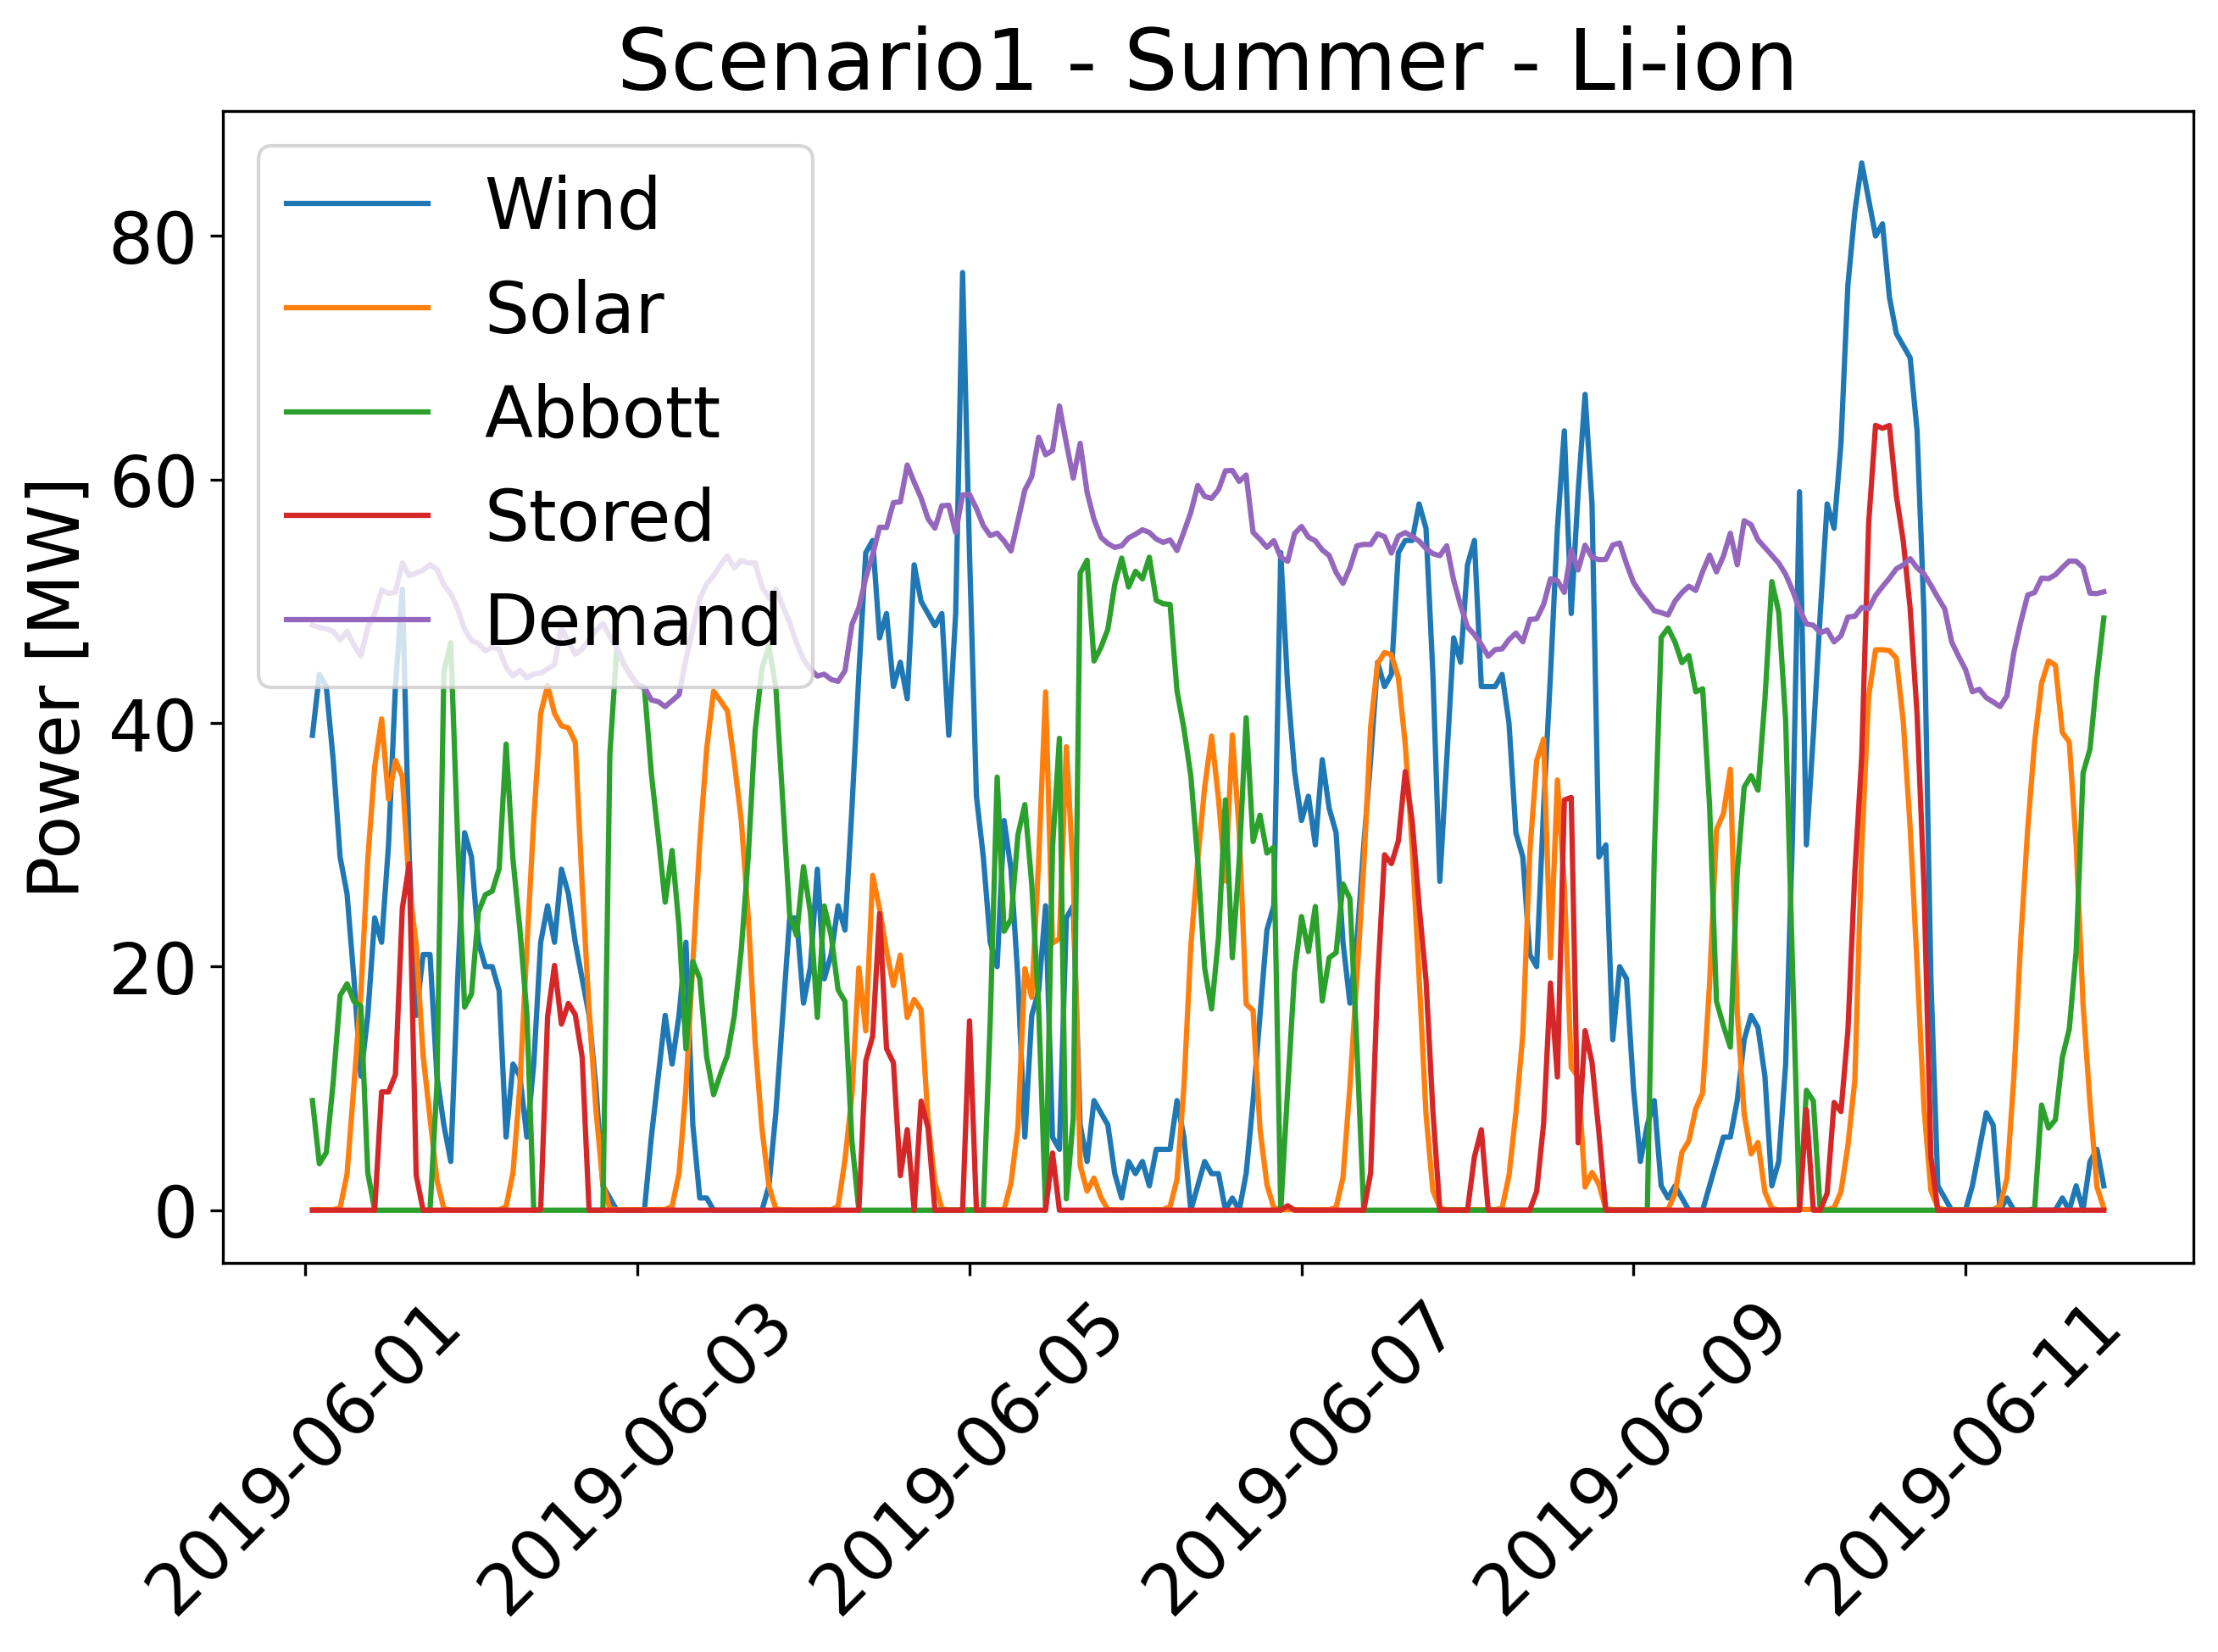
\includegraphics[width=0.90\linewidth]{figures/scenario1-summerB2}
    \hfill
    \caption{Scenario 1 hourly generation distribution by source for a capacity increase factor of 10. Displayed data span from June 1st to June 11th.}
    \label{fig:1-summer-distrib}
\end{figure}

% Scenario 1
Figure \ref{fig:1-summer-distrib} displays an example of the hourly distribution calculated by the dispatch model for Scenario 1.
Subtracting the wind and solar generation from the demand allows calculating the stored electricity, Abbott production, and the purchased electricity.
This figure shows that Abbott has enough capacity to supply campus without the need for purchasing electricity.
This study focuses on the reduction of the CO$_2$ emissions and not on the economics.
Eliminating the electricity purchases already reduces the emissions by almost a half, as shown in Figure \ref{fig:1-summer-emissions}.

% Figure - Scenario 1 - CO2 emissions / Capacities
\begin{figure}[htbp!] %or H 
    \centering
    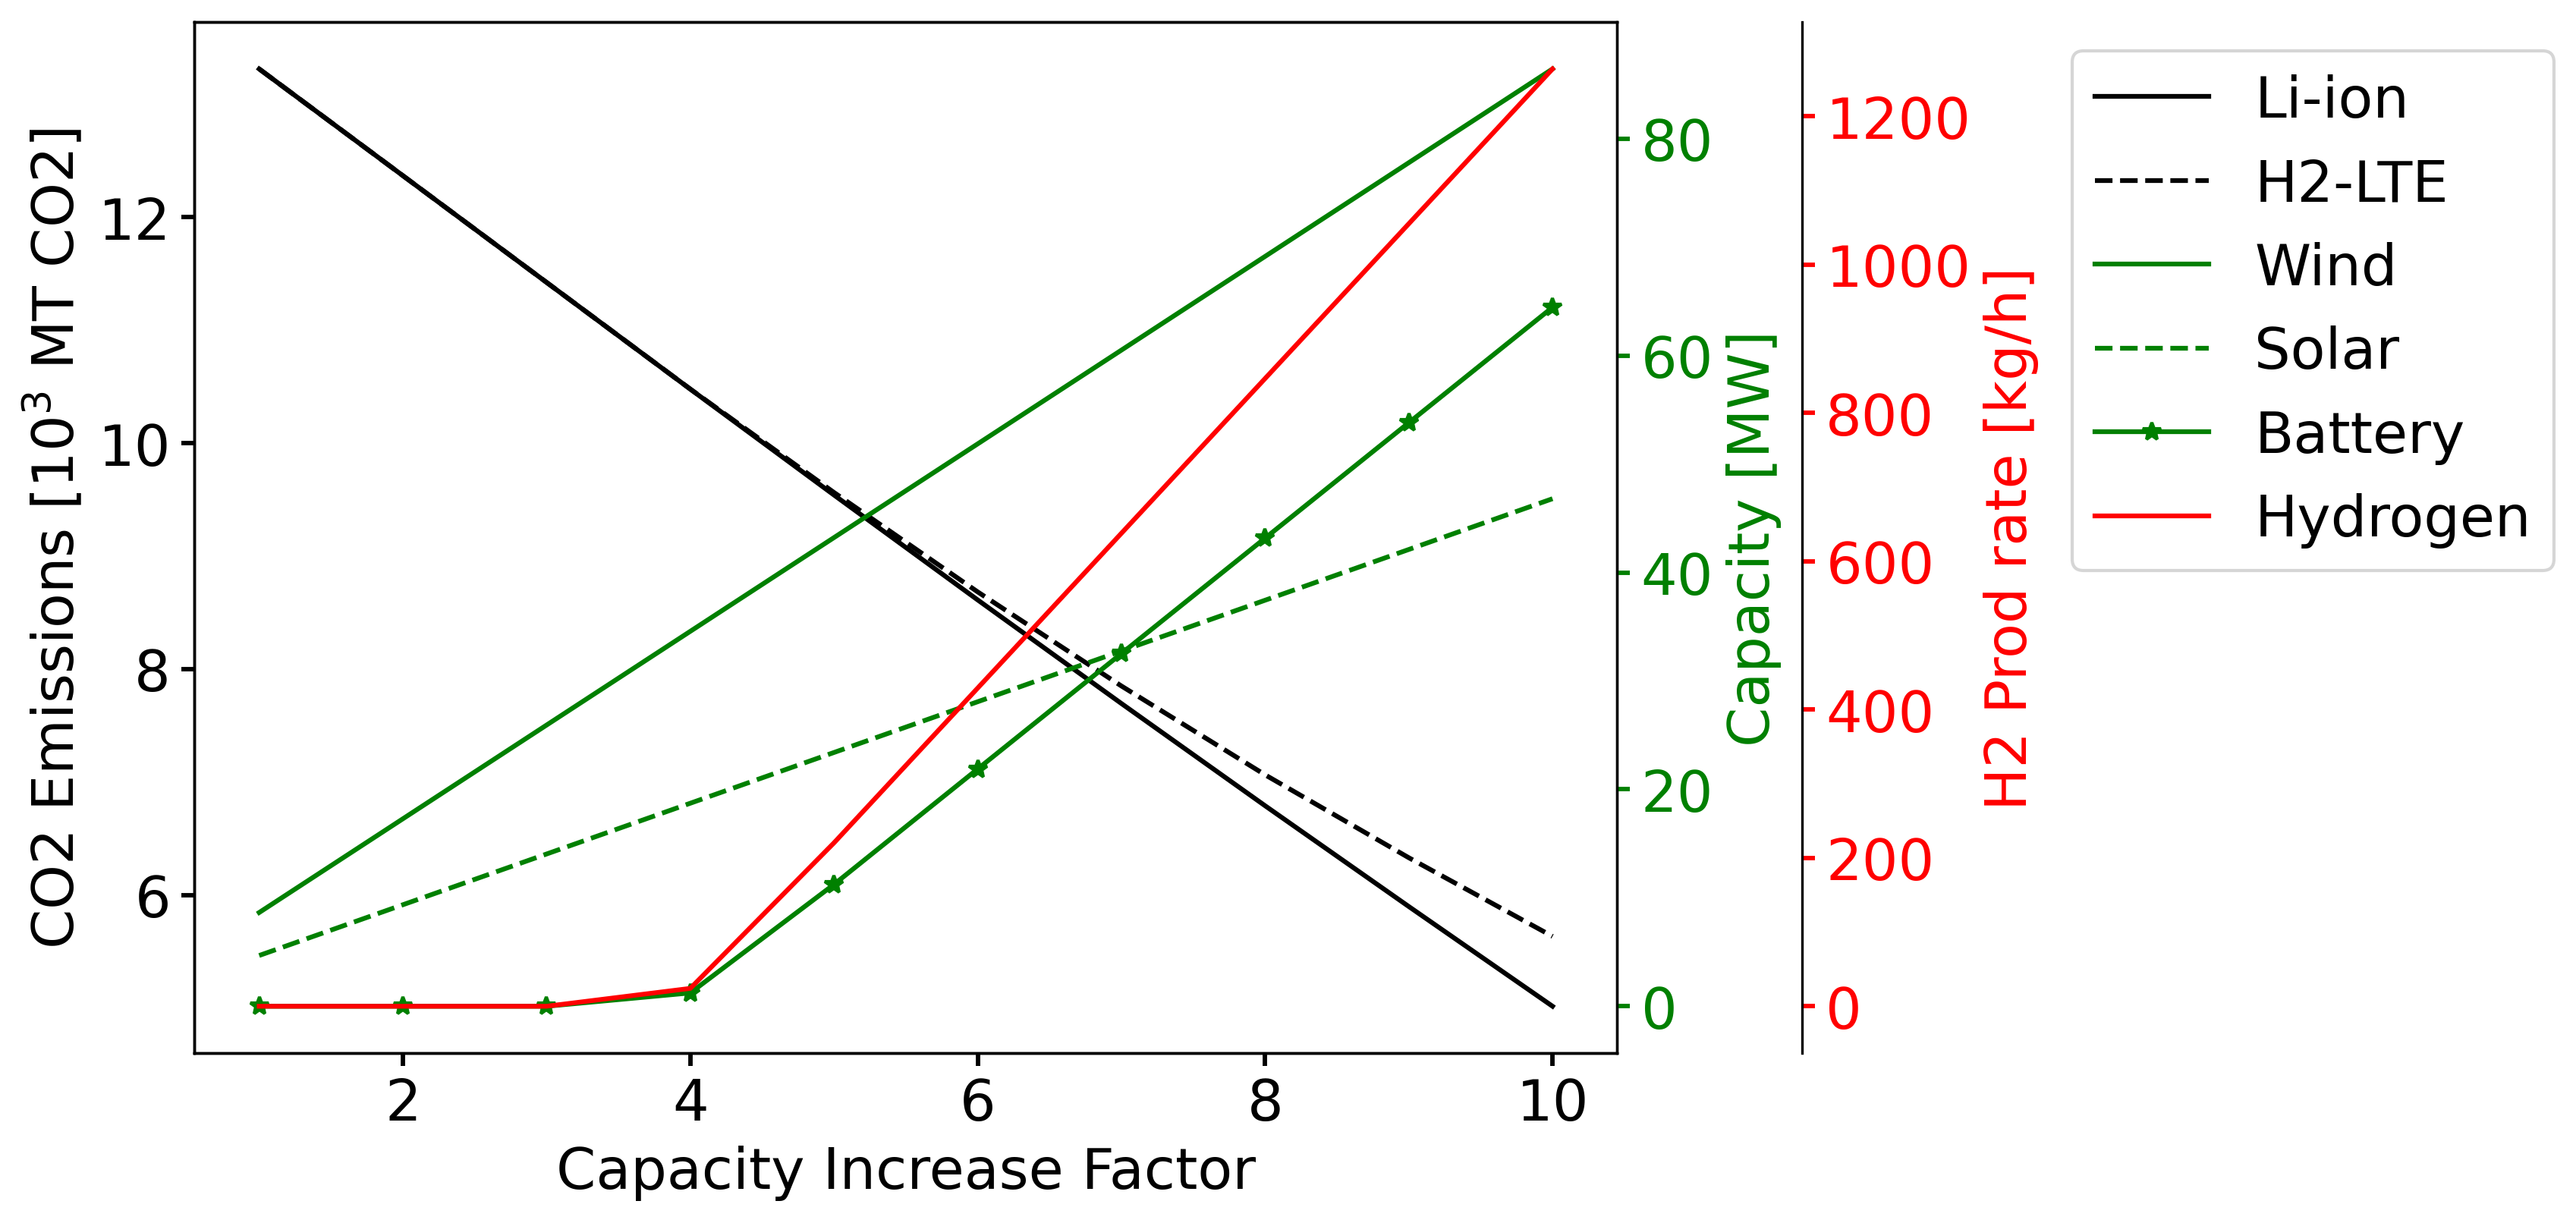
\includegraphics[width=0.99\linewidth]{figures/scenario1-summerA}
    \hfill
    \caption{Scenario 1 CO$_2$ emissions for different increases in the wind and solar generation capacities.}
    \label{fig:1-summer-emissions}
\end{figure}

Figure \ref{fig:1-summer-emissions} displays the CO$_2$ emissions as well as wind, solar, and storage capacities for the different capacity increase factors.
Scenario 1 considers a linear increase in the wind and solar capacities.
Hence, the CO$_2$ reduction is also linear as long as no energy storage is required.
The campus wind and solar capacities can be increased up to 25.9 and 14 MW (increase factor of 3), respectively, without a need for installing a storage mechanism.
Once the energy storage is needed, the higher the charge-discharge efficiency, the larger the emissions reduction is.
This scenario achieves a higher CO$_2$ reduction employing Li-ion batteries.

% Scenario 2
Figure \ref{fig:2-summer-10-emissions} shows the CO$_2$ emissions and the respective wind, solar, and storage capacities for the different capacity increase factors considering a reactor power of 10 MW$_{th}$.
Once again, the Li-ion batteries cause the largest reduction in CO$_2$ emissions.
On the other hand, increasing the solar and wind capacity by a factor of 10 requires Li-ion batteries with larger capacities than the wind generation or the solar generation, being close to 100 MW, which is even larger than the campus total demand.

% Figure - Scenario 2 - CO2 emissions / Capacities for a 10 MWth-Reactor
\begin{figure}[htbp!] %or H 
    \centering
    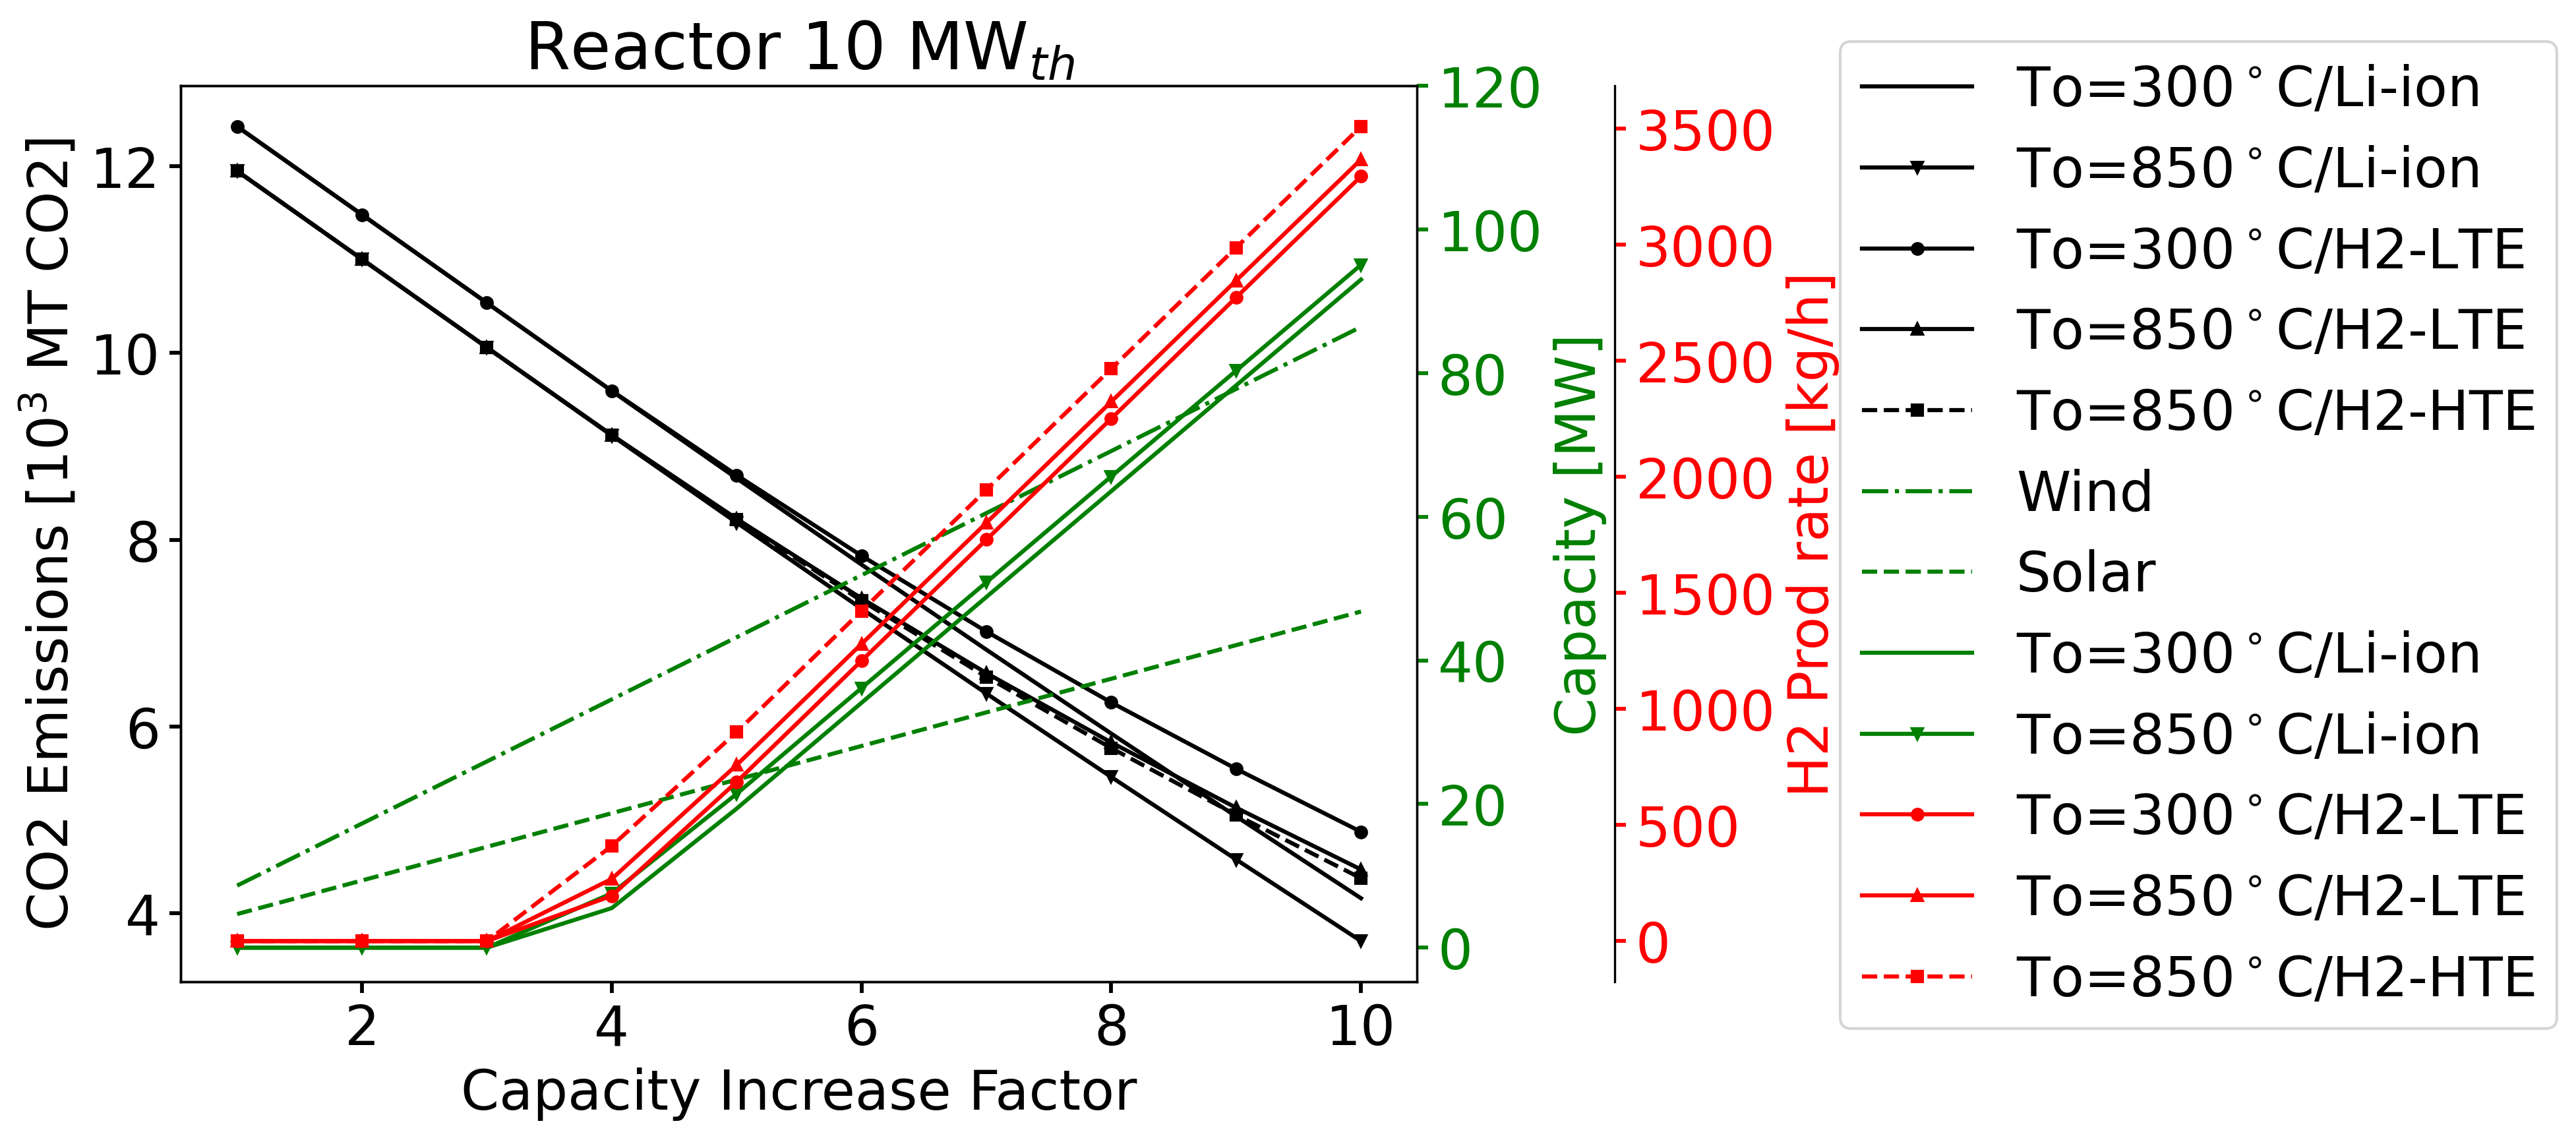
\includegraphics[width=0.99\linewidth]{figures/scenario2-10-summer-emissions}
    \hfill
    \caption{Scenario 2 CO$_2$ emissions for different increases in the wind and solar generation capacities, with a 10 MW$_{th}$ reactor. $To$ is the reactor outlet temperature.}
    \label{fig:2-summer-10-emissions}
\end{figure}

As mentioned earlier, a higher reactor outlet temperature translates into higher efficiencies, and for the same reactor thermal power, a higher electrical output can be achieved.
H2-HTE does not show considerable advantages over H2-LTE, highlighting that a high outlet temperature is still desirable but only for attaining higher efficiencies.
Additionally, incorporating a 10 MW$_{th}$ microreactor reactor reduces the CO$_2$ emissions but does not eliminate them.

% Figure - Scenario 2 - CO2 emissions / Capacities for a 20 MWth-Reactor
\begin{figure}[htbp!] %or H 
    \centering
    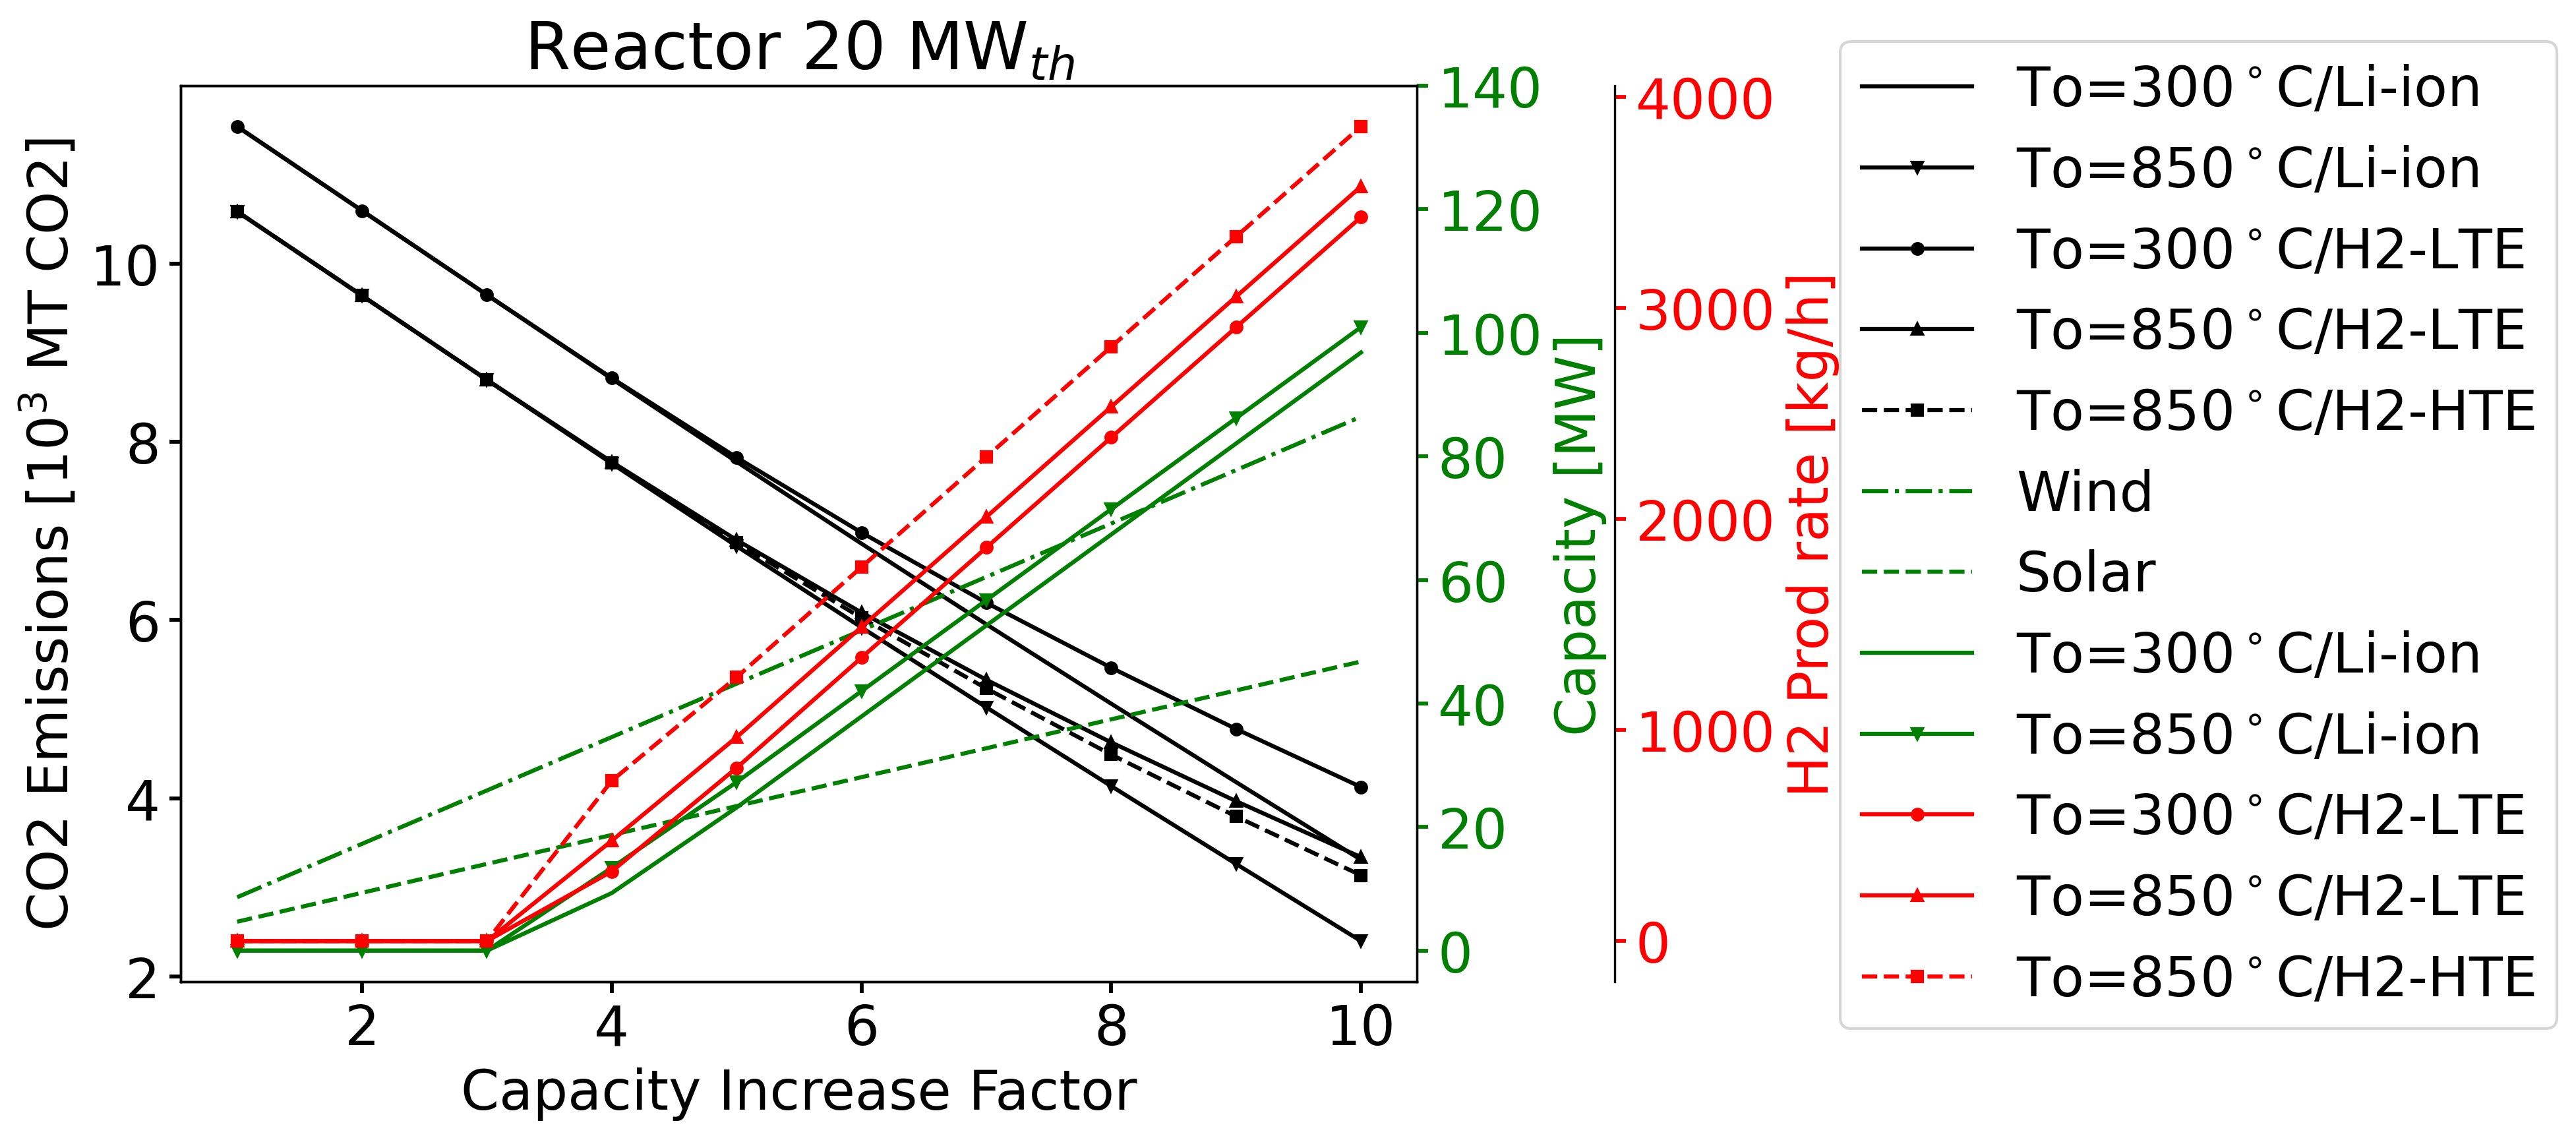
\includegraphics[width=0.99\linewidth]{figures/scenario2-20-summer-emissions}
    \hfill
    \caption{Scenario 2 CO$_2$ emissions for different increases in the wind and solar generation capacities, with a 20 MW$_{th}$ reactor. $To$ is the reactor outlet temperature.}
    \label{fig:2-summer-20-emissions}
\end{figure}

Figure \ref{fig:2-summer-20-emissions} displays the results for the case considering a reactor of 20 MW$_{th}$.
The Li-ion batteries show the best performance.
A higher reactor power translates into a higher CO$_2$ reduction.
Additionally, a higher reactor power allows for an increase in hydrogen production, and the H2-LTE and the H2-HTE curves show a wider separation.


\section{Conclusions}

The world faces energy challenges that compromise the efforts to stop climate change, being the electricity generation sector a major contributor to GHG emissions.
These challenges underscore the need for cleaner sources.
Nonetheless, the common belief that renewable energy is the solution to the problem highlights a caveat.
A stand-alone increase in wind and solar generation capacities cannot eliminate all the carbon emissions.
Such a strategy requires the addition of energy storage mechanisms into the grid.

This work studies several energy alternatives for decarbonizing the UIUC campus grid, including a variety of energy storage mechanisms.
The UIUC campus grid is a good example of a diverse micro-grid, in which different energy sources need to work symbiotically to fulfill campus demand.
This work focused on reducing the carbon emissions on campus, contemplating several approaches.

One of the main takeaways from Scenario 1 is that decreasing the electricity purchases has a strong impact on CO$_2$ emissions.
However, this work considers that Abbott has a maximum capacity of 85 MW and that all that capacity is available if needed. As a co-generation plant, Abbott’s steam production may limit the maximum available electric capacity, requiring the purchase of electricity.
Additionally, the results showed that increasing the capacity of the renewable sources linearly decreases CO$_2$ emissions as long as no storage mechanism is needed.

Concerning Scenario 2, larger reactor capacities reduce further the CO$_2$ emissions.
Additionally, a reactor with higher outlet temperatures increases the total electrical capacity and reduces even further the CO$_2$ emissions.
Finally, Li-ion batteries are the most efficient storage mechanism for all the study cases.


\section{Acknowledgements}

I would like to thank Sam Dotson and Lucas Woodrich for putting together most of the raw data used in this work.
% This research was performed using funding received from the DOE Office of Nuclear Energy’s University Program (Project 20-19693, DE-NE0008972) ’Evaluation of micro-reactor requirements and performance in an existing well-characterized micro-grid’.


%%%%%%%%%%%%%%%%%%%%%%%%%%%%%%%%%%%%%%%%%%%%%%%%%%%%%%%%%%%%%%%%%%%%%%%%%%%%%%%%
\bibliographystyle{ans}
\bibliography{bibliography}
\end{document}

% \begin{figure}[htbp!] %or H 
%     \centering
%     \includegraphics[width=0.95\linewidth]{figures/radial-layout.png}
%     \hfill
%     \caption{Core radial layout. Image reproduced from \cite{oecd_nea_benchmark_2017}.}
%     \label{fig:radial}
% \end{figure}

% \begin{align}
%     \frac{1}{v_g}\frac{\partial}{\partial t} \phi_g &= \nabla \cdot D_g
%     \nabla \phi_g - \Sigma_g^r \phi_g \sum_{g \ne g'}^G
%     \Sigma_{g'\rightarrow g}^s \phi_{g'} \label{eq:diffusion}
%     \intertext{where}
%     C_i &= \mbox{concentration of delayed neutron precursors} \notag \\
%     &\phantom{{}=1} \mbox{in precursor group $i$}.
% \end{align}

% \subsection{Mathematical Basis}
% % Boussinesq approximation
% \begin{align}
% \rho \left[ \frac{\partial \vec{u}}{\partial t} + (\vec{u} \cdot \nabla)\vec{u} \right] &= - \nabla p + \mu \nabla^2 \vec{u} - \rho \vec{g} \\
% \rho &= \rho_0 \left[ 1-\beta(T-T_0) \right] ^ \beta = \frac{1}{T_{ref}} \\
% \rho_0 \left[ \frac{\partial \vec{u}}{\partial t} + (\vec{u} \cdot \nabla)\vec{u} \right] &= - \nabla p + \mu \nabla^2 \vec{u} - \rho_0 \vec{g} \beta (T-T_0)
% \end{align}
